\documentclass[12pt]{article}

% ---------- Packages ----------
\usepackage[utf8]{inputenc}     % UTF-8 encoding
\usepackage[T1]{fontenc}        % Better font encoding
\usepackage{lmodern}            % Improved font rendering
\usepackage[margin=1in]{geometry} % 1-inch margins
\usepackage{setspace}           % Line spacing
\usepackage{parskip}            % No indent, spacing between paragraphs
\usepackage{graphicx}           % For including images
\usepackage[font=small,labelfont=bf]{caption}            % Better captions
\usepackage{subcaption}         % Subfigures
\usepackage{float}              % Improved float handling
\usepackage{amsmath, amssymb}   % Math packages (if needed)
\usepackage{mathtools}
\usepackage{booktabs}           % Better tables
\usepackage{hyperref}           % Clickable links
\usepackage{fancyhdr}           % Headers and footers
\usepackage{enumitem}           % Better lists
\usepackage[backend=biber,style=mla]{biblatex} % APA citations (adjust if needed)
\usepackage{graphicx}
\usepackage{siunitx}
\usepackage{tikz}
\usepackage{tabularx}
\usepackage{pgfplots}
\usepackage[version=3]{mhchem}
\usepackage{pdftexcmds}
\usepackage{chemfig}
\usepackage{array}
\usepackage{makecell}
\usepackage{cleveref}
\usepackage{multirow}
\pgfplotsset{compat=1.18}
\usepackage{listings}
\usepackage{xcolor}




\newcolumntype{Y}{>{\centering\arraybackslash}X}


% ---------- Bibliography ----------
\addbibresource{references.bib}  % Create this file for your sources

% ---------- Line Spacing ----------
\doublespacing

% ---------- Document ----------


\begin{document}
	
	\begin{titlepage}
		\centering
			\textbf{Internal Assessment \textemdash\ Geography SL}
			
			\vspace*{1.5cm}
			
				% Title
			{\Huge \bfseries To what extent does the River Modau conform to the Bradshaw Model? \par}
			\vspace{2cm}
		
			% Cover image
		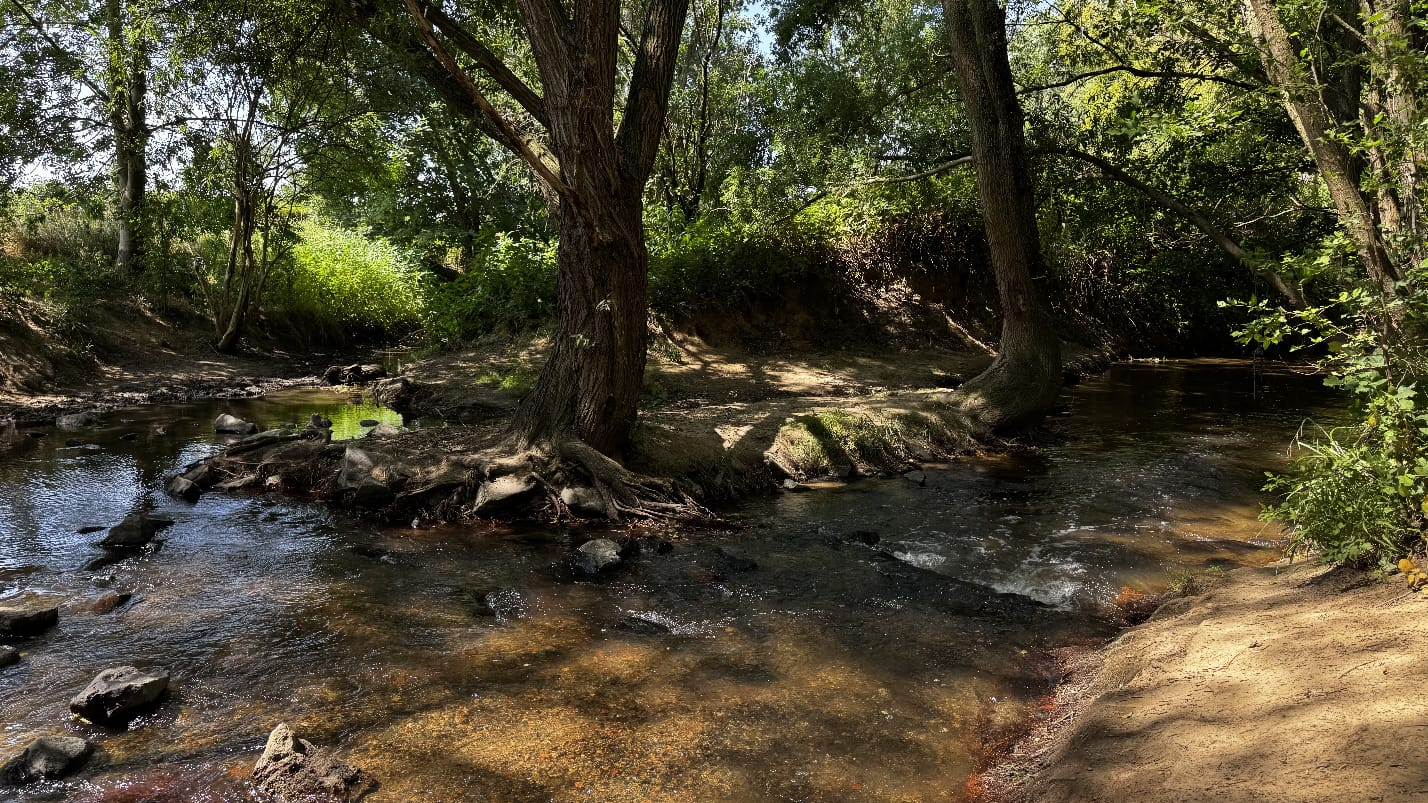
\includegraphics[width=0.7\textwidth]{Images/Cover_page_picture.jpg}\par\vspace{1.5cm}

		% Candidate Code
		{\large Candidate Code: \par}
		\vspace{0.5cm}
		
		Word count:\\
		
	\end{titlepage}
	
	\tableofcontents
	\section{Introduction}
\label{sec:intro}

\subsection{Modau River}

The Modau River is a small river located in the state of Hesse, Germany. Geographically, it originates in the Odenwald hills near Neunkirchen and flows northwest through a series of valleys and lowlands. The river stretches approximately 44 kilometres before it empties into the Rhine River near Stockstadt am Rhine. As it flows through town like Ober-Ramstadt, Pfungstadt, and parts of Darmstadt, the Modau shapes the surrounding landscape by contributing to the local drainage system and influencing soil fertility. Its drainage basin lies within a temperate climate zone, and the river plays a role in regional hydrology, especially in terms of groundwater surface-water runoff.

\begin{figure}[H]
	\centering
	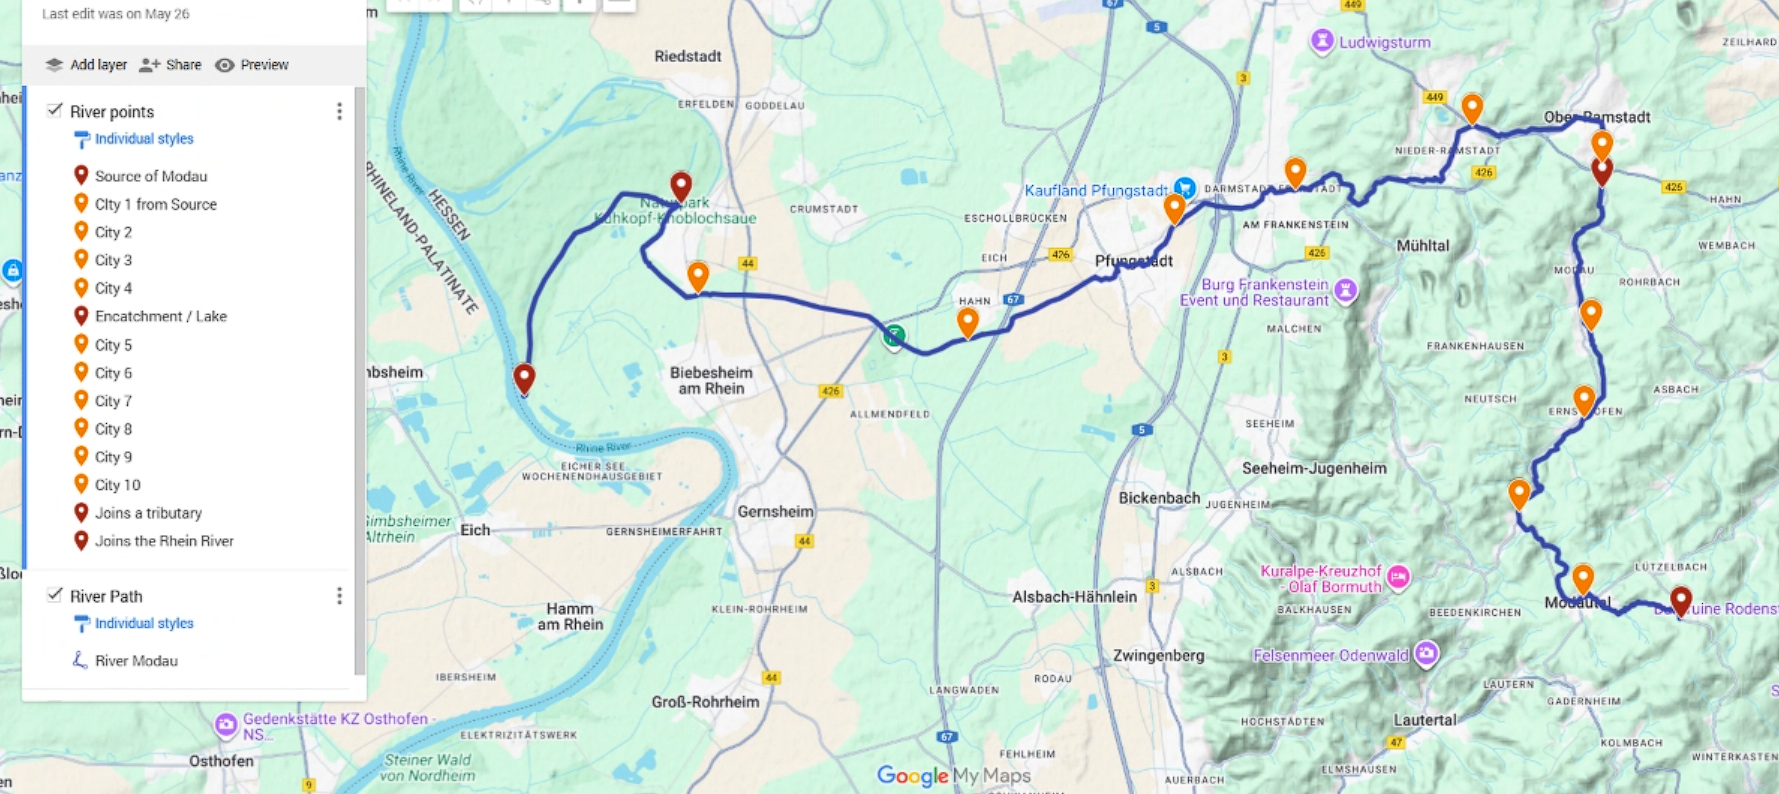
\includegraphics[width=0.9\textwidth]{Images/Selfmade_map_Modau.png}
	\caption{Map of Modau and towns and cities located on/near it using \textcite{googlemaps_darmstadt}.}
\end{figure}

As shown in the map, one can clearly follow the tributary from its source in the hills to the east, its upper course till Ober-Ramstadt where the river path is straight and in a v-shape valley, its middle course till Pfungstadt where it has entered its flat-floored valley leaving behind the hills with slight meanders which are more prominent when zoomed, and finally, the lower course as it joins the Rhine River. Here it is clearly a flat valley as the beige colour represents the surrounding farmland by the river. Meanders are clearer and more visible. As it flows to the River Rhine, the Modau has tributaries that flow into it the more we descend in altitude.

\subsection{Bradshaw Model}

\begin{figure}[H]
	\centering
	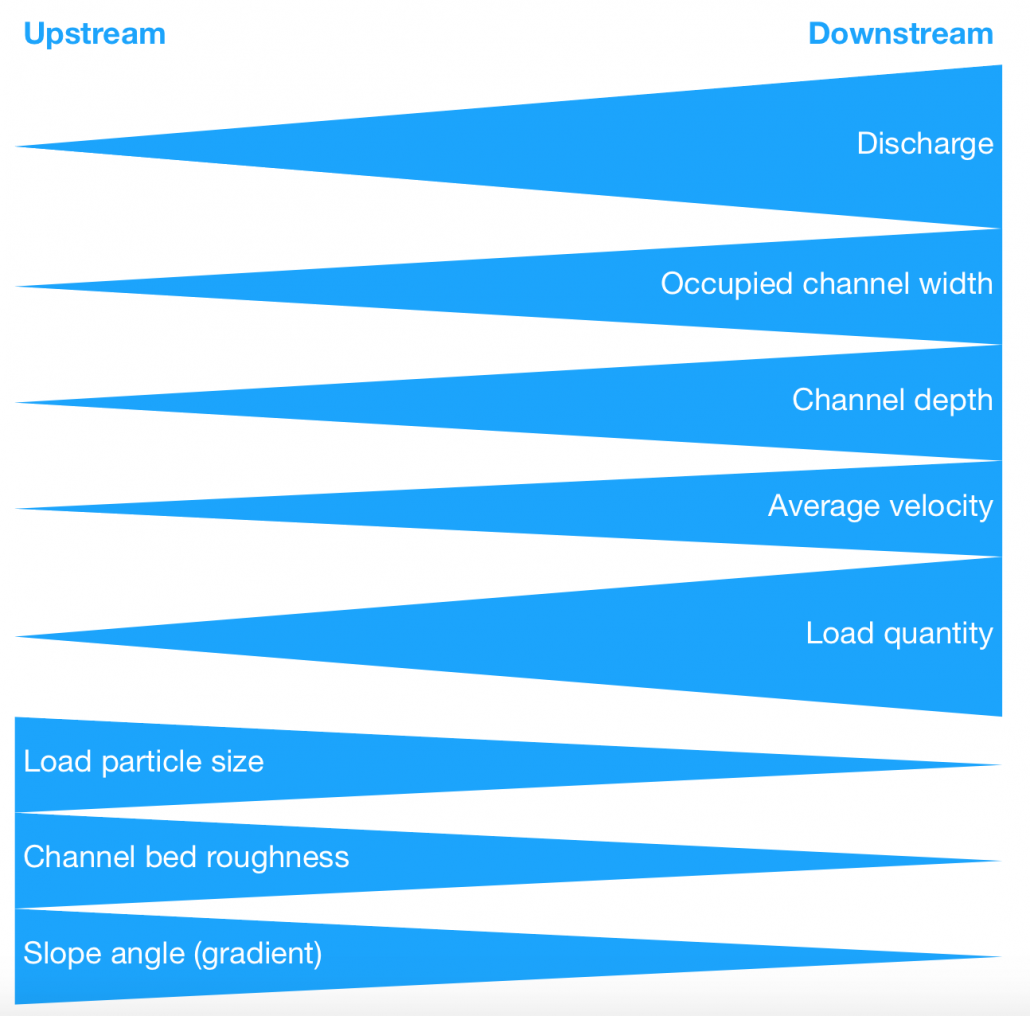
\includegraphics[width=0.65\textwidth]{Images/Bradshaw_Model.png}
	\caption{\textcite{internetgeography_riverfieldwork}}
\end{figure}

The Bradshaw Model is a geographical model which theorizes the characteristics of a river, stream, or tributary as one moves downstream from the source to the mouth \parencite{enacademic_weir}. However, the model can be read from both ways, upstream and downstream. Here it portrays how river discharge, channel width, depth, average velocity, and load quantity increase as one proceeds downstream. On the other hand, moving down stream, the load particle size, channel bed roughness, and gradient decrease \parencite{coolgeography_channelcharacteristics}. Despite showing the predicted river characteristics moving downstream, the Bradshaw Model does not encompass all the features of the river. Properties such as channel efficiency, river valley shapes and river landforms are exempt from this paradigm.

\subsection{Aim}

The aim of this following investigation is to determine the accuracy of the Bradshaw Model in predicting the characteristics of a river as it flows from its source down to its mouth.

\section{Hypotheses}
\label{sec:hypotheses}

\vspace*{0.5cm}


\begin{enumerate}
	\item As you move downstream, the velocity increases as channel efficiency increases. 
	\item As one moves downstream there is an increase in channel width and channel depth, the river discharge also increases.     
	\item Bedload size will decrease as we go downstream.
\end{enumerate}


	\section{Hypotheses}
\label{sec:hypotheses}

\vspace*{0.5cm}


\begin{enumerate}
	\item As you move downstream, the velocity increases as channel efficiency increases. 
	\item As one moves downstream there is an increase in channel width and channel depth, the river discharge also increases.     
	\item Bedload size will decrease as we go downstream.
\end{enumerate}


	\section{Methodology}
\label{sec:method}


\subsection{Velocity (Digital)}

\begin{figure}[H]
	\centering
	\makebox[\linewidth][c]{
	\begin{tikzpicture}
		\node[inner sep=0pt] (img) at (0,0) {	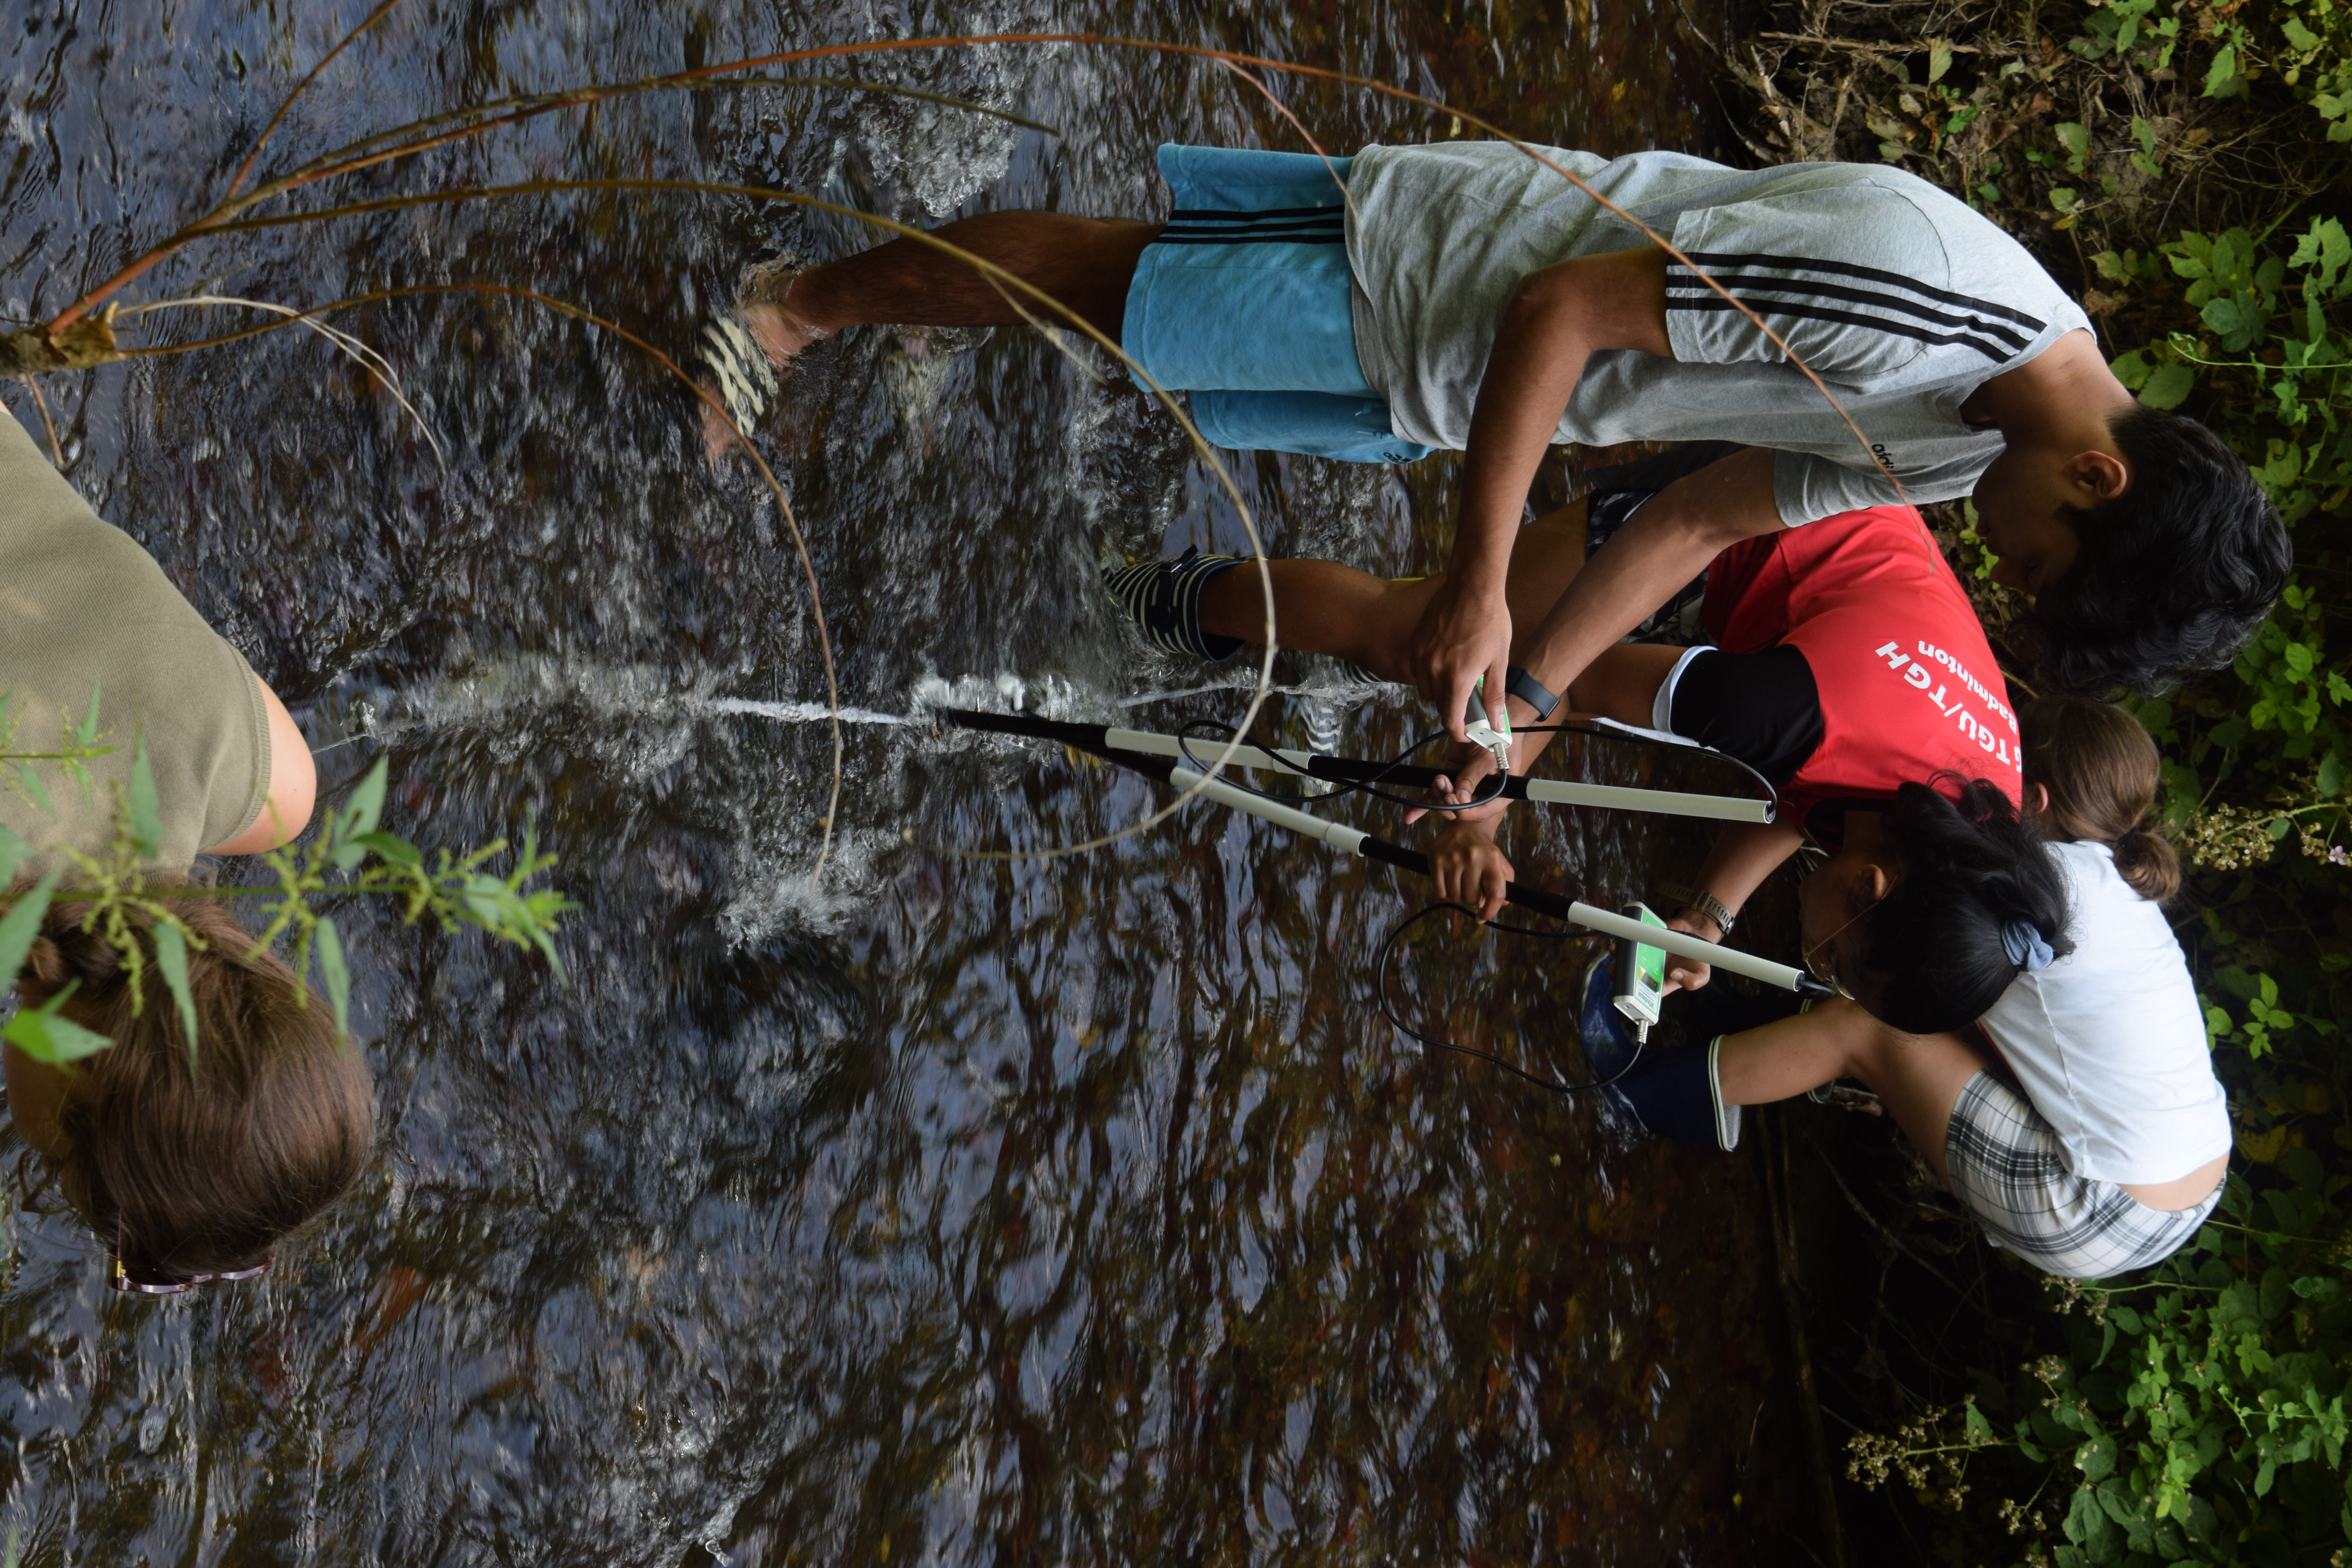
\includegraphics[width=0.7\textwidth, angle=90]{Images/digitalvelo_3.jpg}};
		
		%right
		\draw[->, line width=2pt, color=red] (6.9, 0) -- (-0.35, -0.64);
		\node[draw, fill=white, line width=1pt, anchor=west, align=left] at (7, 0) {Digital Flowmeter};
		
		\draw[->, line width=2pt, color=red] (5.6, 4) -- (0.45, 3.0);
		\node[draw, fill=white, line width=1pt, anchor=west, align=left] at (5.7, 4) {Measured at River \\ Bank along water surface};
		
		%left
		\draw[->, line width=2pt, color=red] (-4.9, 3) -- (-0.28, -1.8);
		\node[draw, fill=white, line width=1pt, anchor=east, align=left] at (-5, 3) {Measuring Tape};
		
			%left
		\draw[->, line width=2pt, color=red] (-4.7, 1) -- (-0.4, -2.5);
		\node[draw, fill=white, line width=1pt, anchor=east, align=left] at (-4.8, 1) {Tape meaure not taut \\ due to high velocity of river \\ exerting force};
		
	\end{tikzpicture}}
	\caption{Digital Velocity measured at Site 3.}
\end{figure}

Velocity was measured in two ways for the following investigation, digital and analogue. To measure digitally, first the width of the river channel was measured at each site and the middle of the channel was recorded. This middle point in the river was where the flow-meter was placed at the surface, with the propeller facing against the flow, in order to measure the velocity as a form of \textbf{purposive sampling}\footnote{\textbf{Purposive sampling} is when a sample is chosen based on a predetermined feature, which is beneficial to the outcome of the study.}.

\clearpage

\[
\textbf{Velocity Equation when digital flow-meter is not used:} 
\]
\[
v = \frac{\Delta s}{\Delta t}
\qquad\qquad
\begin{aligned}
	v &= \text{velocity (m/s)} \\
	\Delta s &= \text{change in distance (m)} \\
	\Delta t &= \text{change in time (s)}
\end{aligned}
\]


Purposive sampling is used, as the least drag is present in the middle of the river channel and away from the river bed, which is a pre-defined characteristic chosen for higher accuracy. This was measured 4 times as the data kept fluctuating by one decimal point, then the average was calculated. A digital flow-meter was used for the data as it is more accurate than an analogue measurements as obstacles in the river, can halt or alter the flow of the float. 

\subsection{Channel Width}

\begin{figure}[H]
	\centering
	\includegraphics[width=1.0\textwidth]{Images/WidthAcc.jpg}
	\caption{Measurement of Channel width in middle course.}
\end{figure}

Measurement of the channel width was taken by using a tape measure. The tape measure was placed perpendicular to river flow and the measurement was taken from river bank to river bank at the points where the water meets the bank. During this the tape measure was pulled taut across the water surface before the measurements were taken. There were 3 measurements made for width and the sampling technique used was pragmatic sampling.

This method of sampling was used as the point in the sites chosen to measure width were chosen as they were the most accessible with the least amount of obstructions, which would cause uncertainties.


\subsection{Channel Depth}

\begin{figure}[H]
	\centering
	\includegraphics[width=0.75\textwidth]{Images/DepthAcc.jpg}
	\caption{Depth measurements taken at river}
	\label{fig:Depth}
\end{figure}

Measurement of the channel depth was taken through the use of a meter rule. A tape measure spanning the width of the river was placed in order to provide the overall width, which would then help determine the intervals at which to measure the depth across the river channel. The meter rule was placed with its narrower side exposed to river flow and the distance between the water surface and the riverbed was measured and recorded. 

Pragmatic sampling was also utilised here as places that had fewer significant protrusions in the river bed, such as large rocks, were avoided to allow for a more accurate measurement of the river bed. These measurements were taken 3 times at each interval and had the average calculated for each of the intervals. Then for the overall depth, the mean of the averages was used.

\subsection{Cross-Sectional Area}

Cross-sectional area is measured by multiplying the mean width with the mean depth.

	\begin{align*}
	A &= \text{Mean Width} \times \text{Mean Depth} \\
	A_{\text{Site 1}} &= 2.02 \times 0.145 = 0.2929 \text{ m$^2$} \\
	\end{align*}
	


\subsection{Channel Efficiency}


\begin{enumerate}
	\item Channel efficiency = Hydraulic radius -> The higher the radius, the greater the efficiency.
	\item $\text{Cross-Sectional Area}\div\text{Wetted Perimeter} = \text{Hydraulic Radius}$
\end{enumerate}


\begin{align*}
	R &= \frac{A}{P} \\
	R_{\text{Site 1}} &= \frac{0.2929}{2.03} = \text{0.144 m (3 s.f.)} \\
\end{align*}

\subsection{River Discharge}

$\text{Discharge (cumecs)}= \text{Cross-Sectional Area}\ (\si{\metre\squared}) \times \text{Velocity}\ (\si{\metre\per\second})$

The mean depth and mean width are first used to measure cross-sectional area (\si{\metre\squared}), then the velocity is measured through either a digital flow-meter or with a stopwatch, a cork,measuring tape and ranging poles ($\times 4$). Then the average velocity is taken and multiplied by the area to get the discharge fo the river.


\begin{align*}
	Q &= A \times \text{v} \\
	Q_{\text{Site 1}} &= 0.2929 \times 0.5725 = 0.168 (3 s.f.) \text{ m$^3$/s} \\
\end{align*}

\subsection{Bedload Size}

\begin{figure}[H]
	\centering
	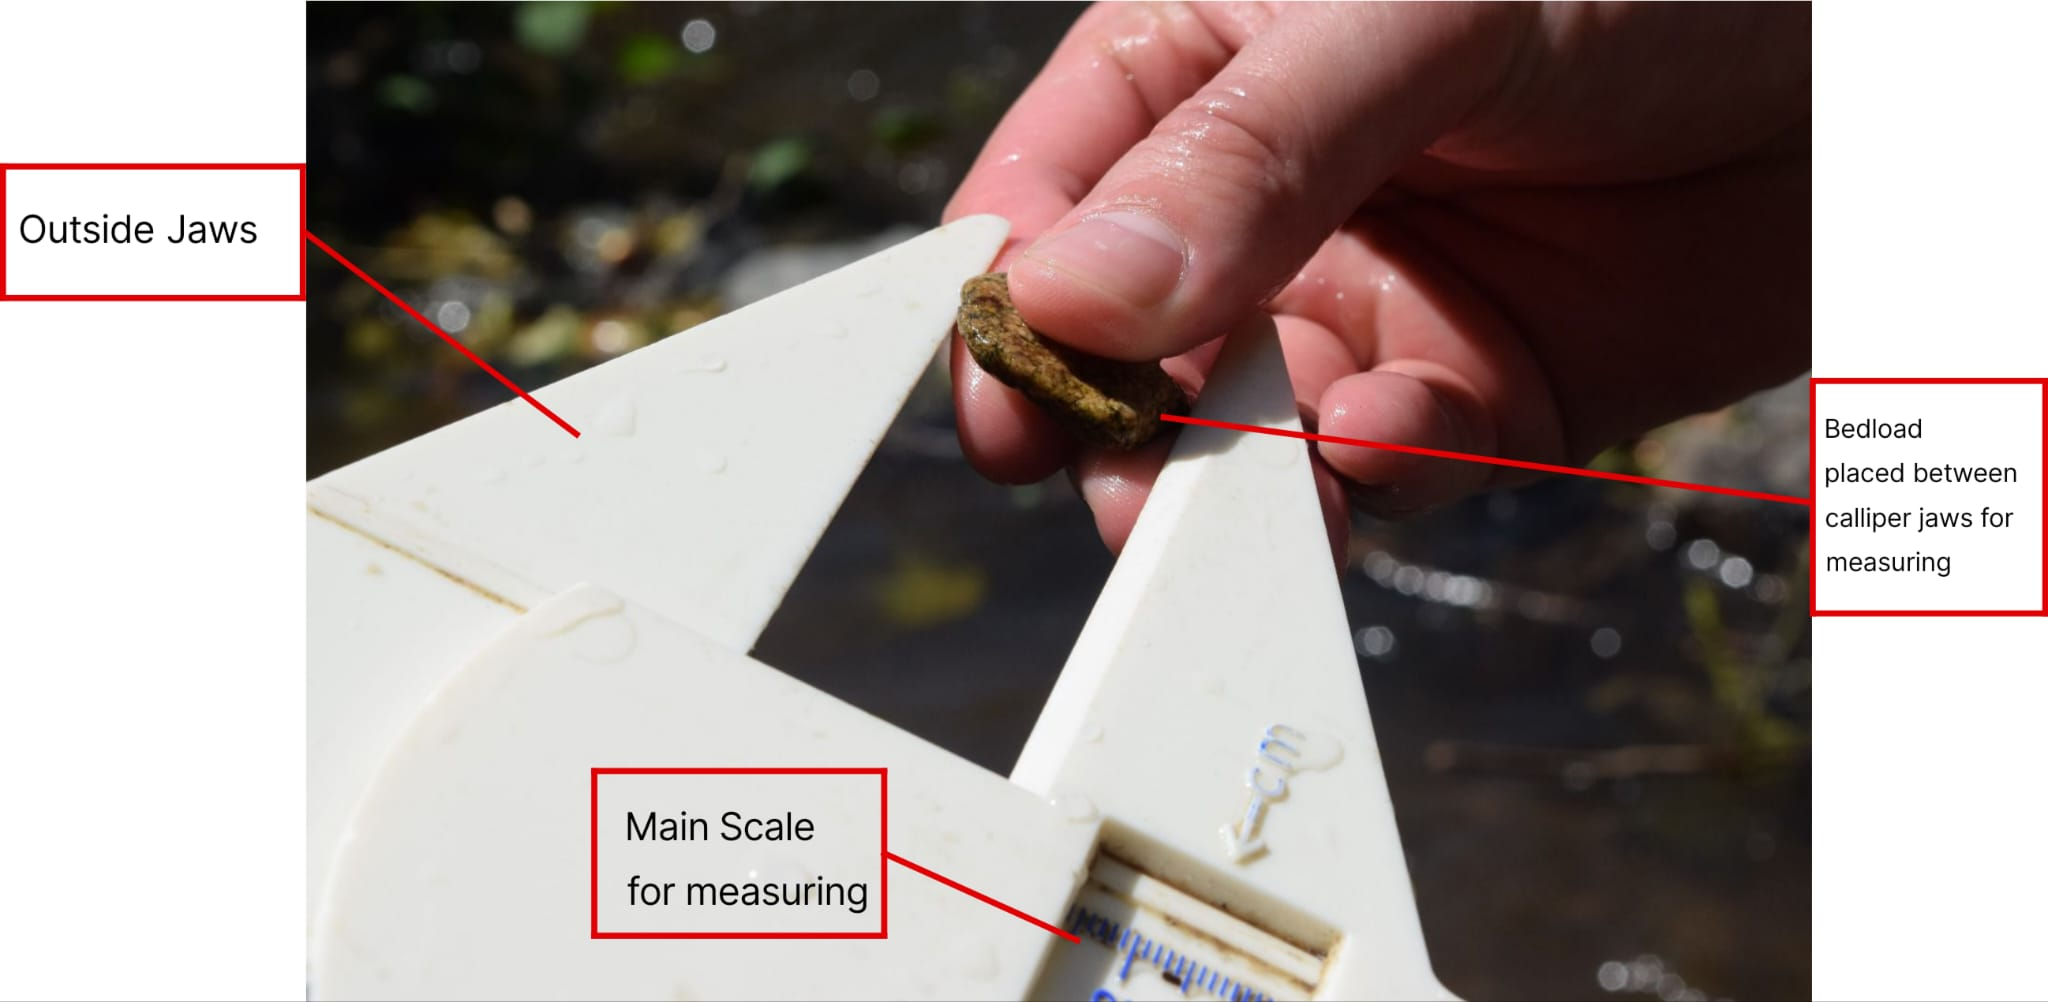
\includegraphics[width=0.9\textwidth]{Images/Bedloadmeasacc.jpg}
\end{figure}

To measure bedload size, a calliper was used and measurements on the chosen rock's length, width and breadth were taken. These results were then averaged and recorded on a table. 10 samples were measure at every site, the averages of the average sizes of these samples were taken in order to determine the average bedload size at each site.

Systematic sampling was used in this case so as to broaden the variety of bedload samples used to be measured in order to provide a higher level of accuracy.




	\section{Processed Data}

\subsection{Velocity}

	\subsubsection{Sample Calculations}
	
	\begin{align*}
		\bar{v} &= \frac{\text{distance traveled by water}}{\text{time taken}} \\
		\bar{v}_{\text{Site 1}} &= 0.5725 \text{ m/s} \\
		\bar{v}_{\text{Site 2}} &= 0.24 \text{ m/s} \\
		&\vdots \\
		\bar{v}_{\text{Site 8}} &= 0.03334 \text{ m/s}
	\end{align*}
	
	\subsubsection{Results}
	
	\begin{figure}[H]
		\centering
		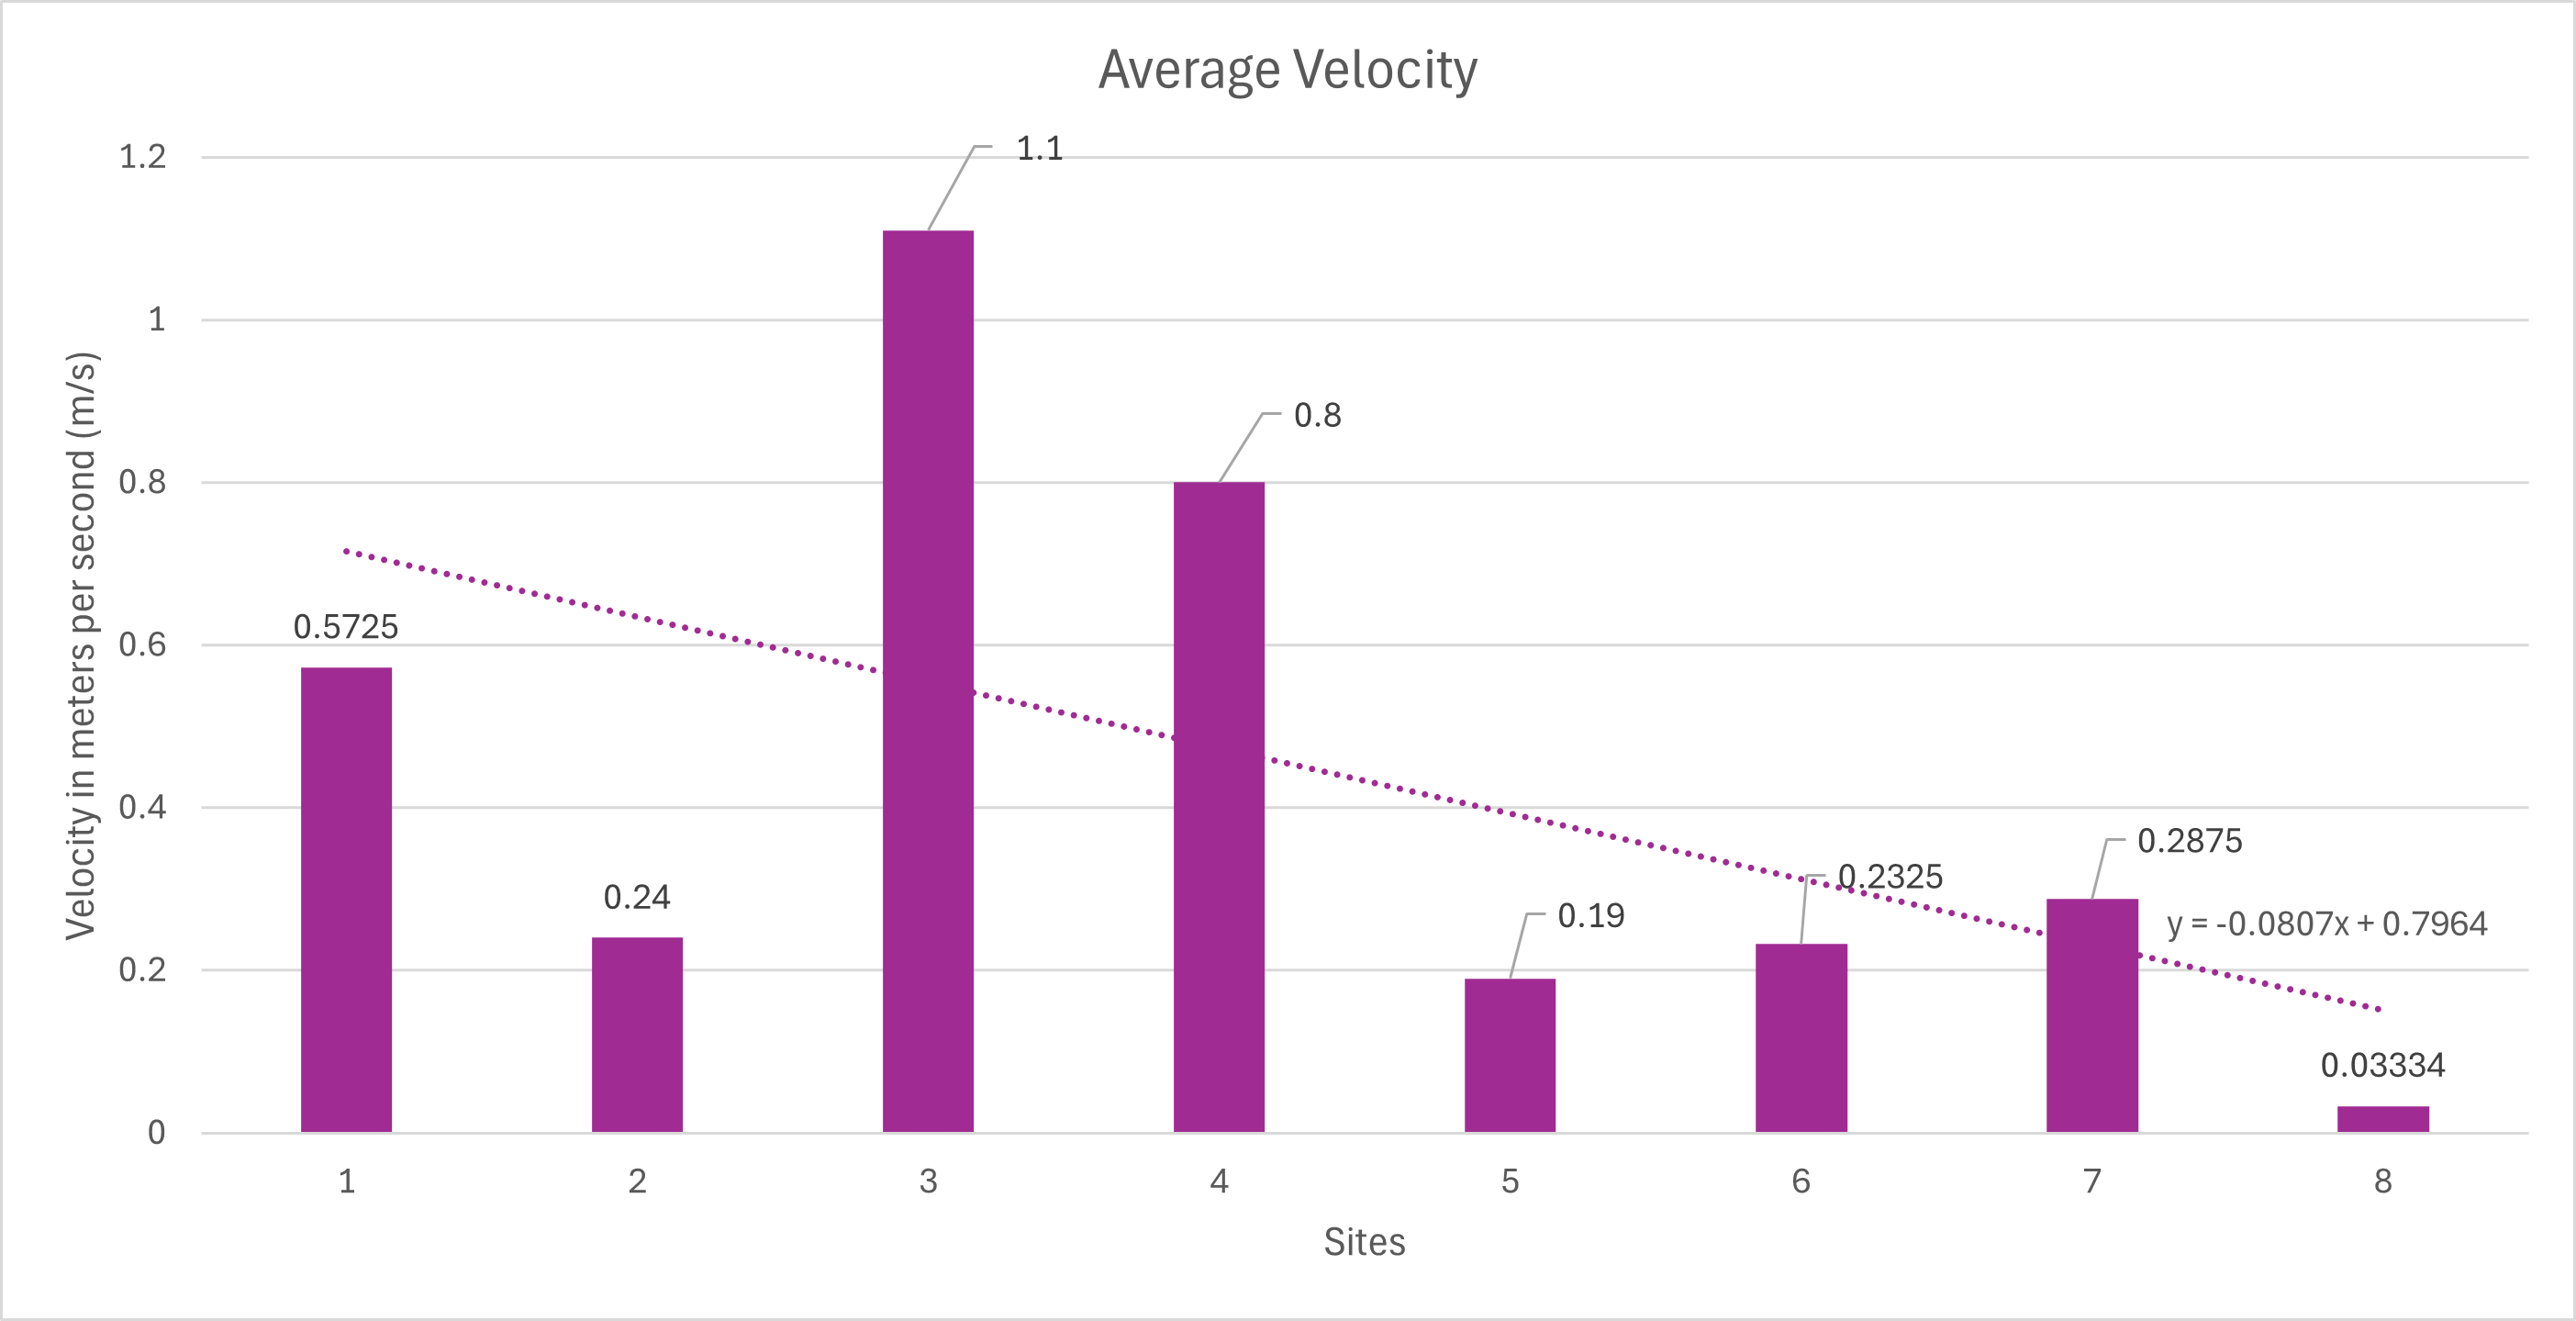
\includegraphics[width=1.0\textwidth]{Images/AverageVelocity.png}
		\caption{Average Velocity at Each Site}
	\end{figure}
	

\subsection{Channel Width}

	\subsubsection{Sample Calculations}
	
	\begin{align*}
		\text{Width} &= \text{measured distance across the water surface at each site} \\
		W_{\text{Site 1}} &= 2.02 \text{ m} \\
		W_{\text{Site 2}} &= 4.19 \text{ m} \\
		&\vdots \\
		W_{\text{Site 8}} &= 4.24 \text{ m}
	\end{align*}

	\subsubsection{Results}

\begin{figure}[H]
	\centering
	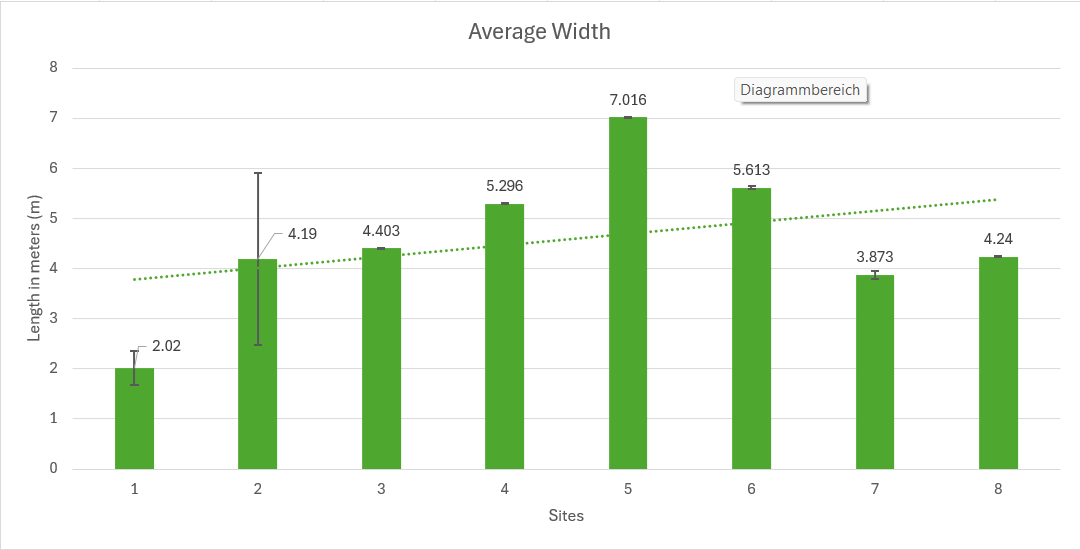
\includegraphics[width=1.0\textwidth]{Images/AverageWidth.png}
	\caption{Average Channel Width at Each Site}
\end{figure}


\subsection{Channel Depth}

	\subsubsection{Sample Calculations}
	
	\subsubsection{Sample Calculations}
	\begin{align*}
		\text{Depth} &= \frac{\text{sum of measured depths at intervals}}{\text{number of measurements}} \\
		D_{\text{Site 1}} &= 0.145 \text{ m} \\
		D_{\text{Site 2}} &= 0.179 \text{ m} \\
		&\vdots \\
		D_{\text{Site 8}} &= 0.280 \text{ m}
	\end{align*}
	
	\subsubsection{Results}

\begin{figure}[H]
	\centering
	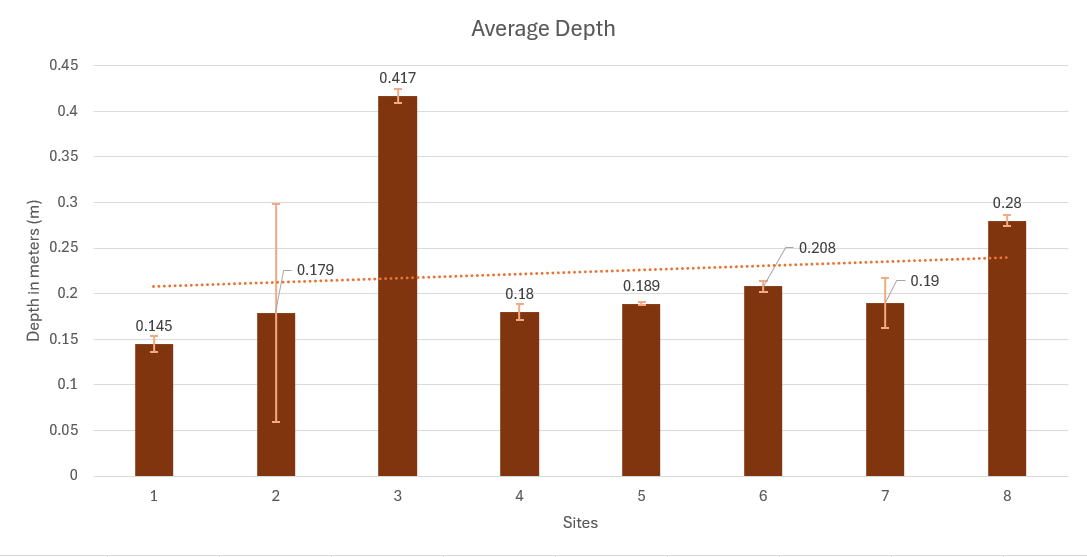
\includegraphics[width=1.0\textwidth]{Images/AverageDepth.png}
	\caption{Average Channel Depth at Each Site}
\end{figure}


\subsection{Wetted Perimeter}

	\subsubsection{Sample Calculations}
	
	\begin{align*}
		P &= \text{sum of the lengths of all wetted edges of the channel} \\
		P_{\text{Site 1}} &= 2.03 \text{ m} \\
		P_{\text{Site 2}} &= 2.96 \text{ m} \\
		&\vdots \\
		P_{\text{Site 8}} &= 4.67 \text{ m}
	\end{align*}
	

	\subsubsection{Results}
	
	% Wetted Perimeter
	\begin{figure}[H]
		\centering
		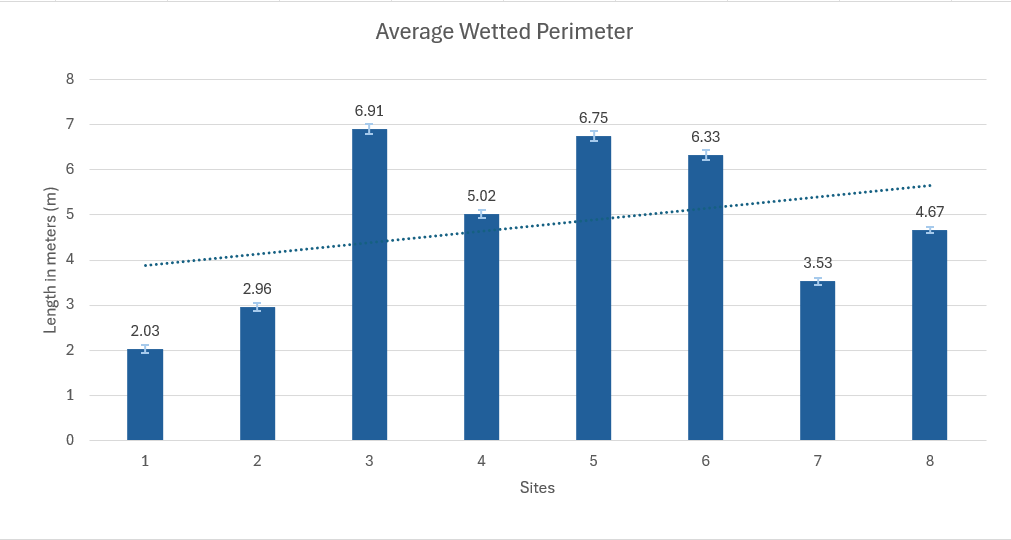
\includegraphics[width=1.0\textwidth]{Images/AverageWettedPerimeter.png}
		\caption{Wetted Perimeter at Different Sites}
	\end{figure}
	
\subsection{Cross-Sectional Area}

	\subsubsection{Sample Calculations}
	
	\begin{align*}
		A &= \text{Mean Width} \times \text{Mean Depth} \\
		A_{\text{Site 1}} &= 2.02 \times 0.145 = 0.2929 \text{ m$^2$} \\
		A_{\text{Site 2}} &= 4.19 \times 0.179 = 0.75001 \text{ m$^2$} \\
		&\vdots \\
		A_{\text{Site 8}} &= 4.24 \times 0.28 = 1.1872 \text{ m$^2$}
	\end{align*}
	

	\subsubsection{Results}
	
	\begin{figure}[H]
	\centering
	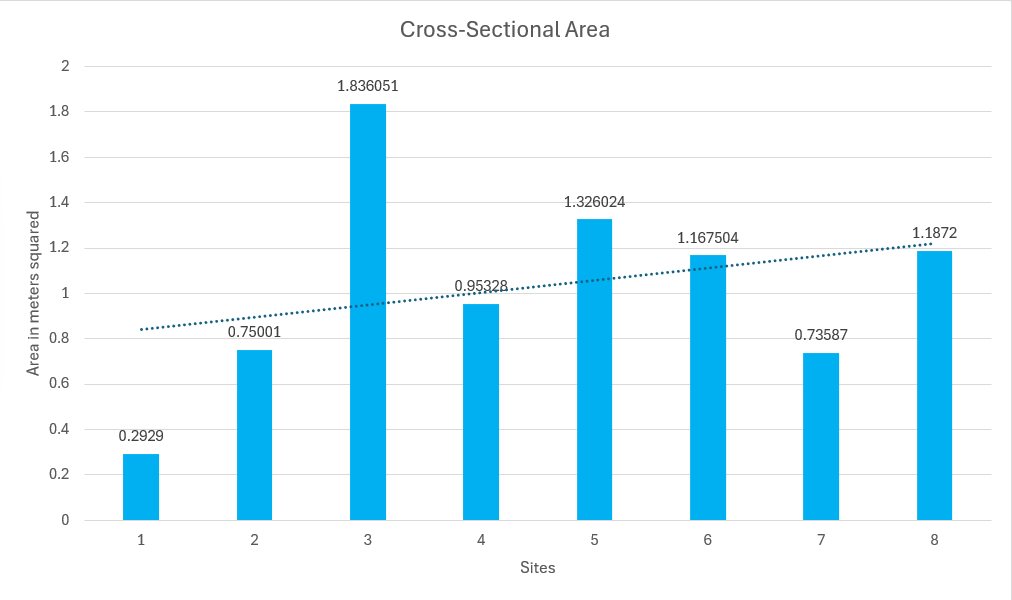
\includegraphics[width=1.0\textwidth]{Images/Cross-SectionalArea.png}
	\caption{Cross-Sectional Area at Different Sites}
\end{figure}

\subsection{Channel Efficiency}

	\subsubsection{Sample Calculations}
	
	%\includegraphics[width=0.7\textwidth]{Images/xx.jpg}\par\vspace{1.5cm}
	
	\begin{enumerate}
		\item Channel efficiency = Hydraulic radius -> The higher the radius, the greater the efficiency.
		\item $\text{Cross-Sectional Area}\div\text{Wetted Perimeter} = \text{Hydraulic Radius}$
	\end{enumerate}
	
	
	\begin{align*}
		R &= \frac{A}{P} \\
		R_{\text{Site 1}} &= \frac{4.08}{2.03} = 2.01 \text{ m} \\
		R_{\text{Site 2}} &= \frac{17.56}{2.96} = 5.932 \text{ m} \\
		&\vdots \\
		R_{\text{Site 8}} &= \frac{17.98}{4.67} = 3.85 \text{ m}
	\end{align*}
	
		\subsubsection{Results}
		
		\begin{table}[H]
			\centering
			\begin{tabularx}{\textwidth}{l *{3}{Y}}
				\hline
				Sites & Wetted Perimeter $P$ (m) & Cross-sectional Area $A$ (m$^2$) & Channel Efficiency $R=A/P$ (m) \\
				\hline
				Site 1 & 2.03 & 4.08  & 2.01 \\
				Site 2 & 2.96 & 17.56 & 5.932 \\
				Site 3 & 6.91 & 19.39 & 2.806 \\
				Site 4 & 5.02 & 28.05 & 5.588 \\
				Site 5 & 6.75 & 49.22 & 7.292 \\
				Site 6 & 6.33 & 31.51 & 4.978 \\
				Site 7 & 3.53 & 15.00 & 4.249 \\
				Site 8 & 4.67 & 17.98 & 3.85 \\
				\hline
			\end{tabularx}
			\caption{}
			\label{tab:channel_efficiency}
		\end{table}

% Channel Efficiency
\begin{figure}[H]
	\centering
	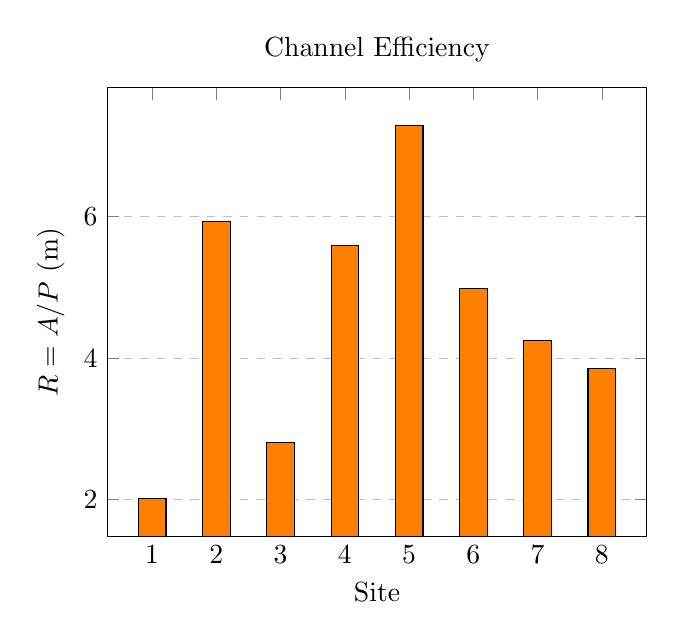
\begin{tikzpicture}
		\begin{axis}[
			title={Channel Efficiency},
			xlabel={Site},
			ylabel={$R=A/P$ (m)},
			xtick=data,
			xticklabels={1,2,3,4,5,6,7,8},
			ymajorgrids=true,
			grid style=dashed
			]
			\addplot[ybar,fill=orange] coordinates {
				(1,2.01) (2,5.932) (3,2.806) (4,5.588) (5,7.292) (6,4.978) (7,4.249) (8,3.85)
			};
		\end{axis}
	\end{tikzpicture}
	\caption{Channel Efficiency at Different Sites}
\end{figure}

\subsection{Discharge}
	
	\subsubsection{Sample Calculations}
	
	\subsection{River Discharge}
	
	\begin{enumerate}
		\item $\text{Discharge (cumecs)}= \text{Cross-Sectional Area}\ (\si{\metre\squared}) \times \text{Velocity}\ (\si{\metre\per\second})$
		\item Use mean depth and mean width to measure cross-sectional area (\si{\metre\squared}).
		\item Measure velocity either through digital flow-meter or with a stopwatch, a cork,measuring tape and ranging poles ($\times 4$)
		\item Then use the average velocity and multiply it by the area to get the discharge
	\end{enumerate}
	
	\begin{align*}
		Q &= A \times \bar{v} \\
		Q_{\text{Site 1}} &= 4.08 \times 0.5725 = 2.34 \text{ m$^3$/s} \\
		Q_{\text{Site 2}} &= 17.56 \times 0.24 = 4.21 \text{ m$^3$/s} \\
		&\vdots \\
		Q_{\text{Site 8}} &= 17.98 \times 0.03334 = 0.60 \text{ m$^3$/s}
	\end{align*}
	
		\subsubsection{Results}
		
		\begin{table}[H]
			\centering
			\begin{tabularx}{\textwidth}{l *{3}{Y}}
				\hline
				Sites & Cross-sectional Area $A$ (m$^2$) & Velocity $\bar{v}$ (m/s) & Discharge $Q=A \times \bar{v}$ (m$^3$/s) \\
				\hline
				Site 1 & 4.08  & 0.5725  & 2.34 \\
				Site 2 & 17.56 & 0.24    & 4.21 \\
				Site 3 & 19.39 & 1.110   & 21.51 \\
				Site 4 & 28.05 & 0.80    & 22.44 \\
				Site 5 & 49.22 & 0.19    & 9.35 \\
				Site 6 & 31.51 & 0.2325  & 7.33 \\
				Site 7 & 15.00 & 0.2875  & 4.31 \\
				Site 8 & 17.98 & 0.03334 & 0.60 \\
				\hline
			\end{tabularx}
			\caption{}
			\label{tab:discharge}
		\end{table}

% Discharge
\begin{figure}[H]
	\centering
	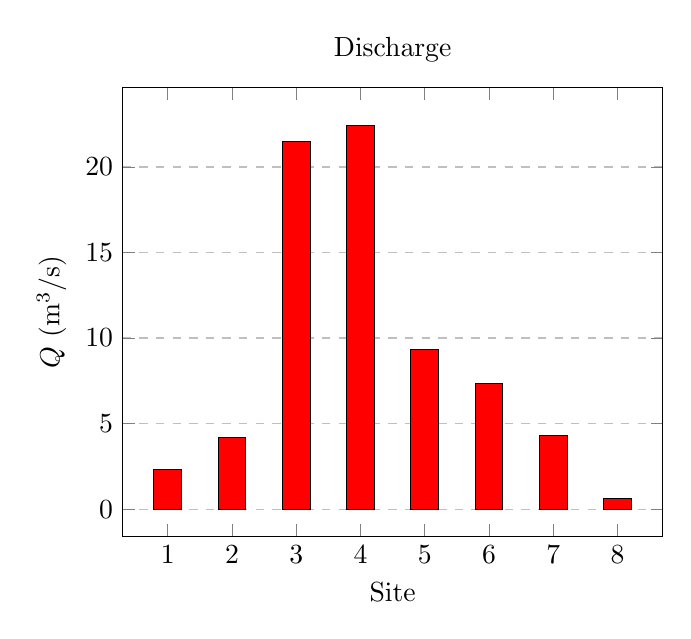
\begin{tikzpicture}
		\begin{axis}[
			title={Discharge},
			xlabel={Site},
			ylabel={$Q$ (m$^3$/s)},
			xtick=data,
			xticklabels={1,2,3,4,5,6,7,8},
			ymajorgrids=true,
			grid style=dashed
			]
			\addplot[ybar,fill=red] coordinates {
				(1,2.34) (2,4.21) (3,21.51) (4,22.44) (5,9.35) (6,7.33) (7,4.31) (8,0.60)
			};
		\end{axis}
	\end{tikzpicture}
	\caption{Discharge at Different Sites}
\end{figure}

\subsection{Bedload Size}

	\subsubsection{Sample Calculations}
	
	\begin{align*}
		\text{Average Bedload Size} &= \frac{\text{Sum of measured sizes}}{\text{Number of particles}} \\
		\text{Site 1} &= 90.20 \text{ mm} \\
		\text{Site 2} &= 84.40 \text{ mm} \\
		&\vdots \\
		\text{Site 8} &= 17.60 \text{ mm}
	\end{align*}
	
		\subsubsection{Results}
		
% Bedload Size
	\begin{figure}[H]
		\centering
		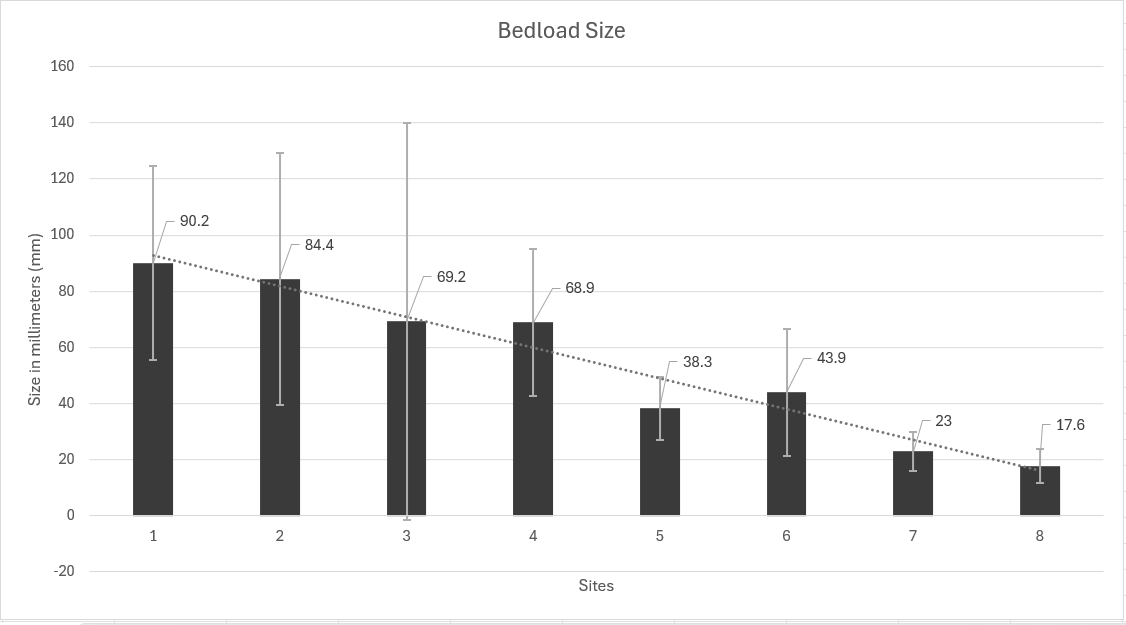
\includegraphics[width=1.0\textwidth]{Images/AverageBedloadSize.png}
		\caption{Bedload Size at Different Sites}
		\end{figure}
		



	\section{Conclusion}

\subsection{Hypothesis 1}

The obtained results vary completely from the expected values as although velocity is supposed to increase as channel efficiency increases, the results show the very opposite happening at all sites except for at Site 8, where the data corresponds to one another. This goes against Bradshaw's model where velocity increases as we move downstream.



\subsection{Hypothesis 2}

As mentioned in the hypothesis, increase in the river's discharge does correlate to the channel width and channel depth to a certain extent. When comparing the discharge with the channel width, one can notice a clear trend with the river discharge increasing as the width increased and the discharge decreasing as the channel width decreased. The only anomaly is at Site 8, where the channel width increases to 4.24 metres in comparison to Site 7 at 3.87 metres, however, the discharge decreases from 4.31 cubic metres per second. Channel width corresponds to Bradshaw's Model where it increases as we move downstream, however, channel depth doesn't support this. Discharge also supports Bradshaw's Model as it shows an increase moving downstream.




\subsection{Hypothesis 3}

Results obtained for the Bedload size completely support the hypothesis that they decrease in size as we move downstream, except for at Site 6, where it increases to 43.9mm from 38.3mm before dropping to 23.0mm at Site 7. More importantly, these results wholly support the Bradshaw Model.
	\section{Evaluation}

There are many reasons for various measurements havng been totally inaccurate due to both natural and man-made causes. Velocity did not match up with Bradshaw's Model at almost all sites due to various hard- and soft-engineering being present. It was high at site 1 due to mattressing present underneath the bridge by site 1, then it slows down at site 2 due to various stones, branches, and other plant material due to its location in the forest. At Site 8, where the river is supposed to be at its fastest, it is at it's slowest, due to build up in sedimentation and silt.


	\section{Appendix}

\subsection{Raw Data}

\begin{table}[H]
	\centering
	\begin{tabularx}{\textwidth}{l *{4}{Y}}
		\hline
		Sites & Recording 1 & Recording 2 & Recording 3 & Recording 4 \\
		\hline
		Site 1 & 0.59 & 0.53 & 0.60 & 0.57 \\
		Site 2 & 0.26 & 0.23 & 0.23 & 0.24 \\
		Site 3 & 0.93 & 1.16 & 1.24 & 1.11 \\
		Site 4 & 0.78 & 0.72 & 0.90 & 0.80 \\
		Site 5 & 0.12 & 0.24 & 0.21 & 0.19 \\
		Site 6 & 0.34 & 0.20 & 0.16 & 0.23 \\
		Site 7 & 0.28 & 0.18 & 0.40 & 0.29 \\
		Site 8 & 0.01 & 0.06 & 0.03 & N/A \\
		\hline
	\end{tabularx}
	\caption{Velocity Digital}
	\label{tab:velocity_digital_raw}
\end{table}

\begin{table}[H]
	\centering
	\begin{tabularx}{\textwidth}{l *{5}{Y}}
		\hline
		Sites & Recording 1 & Recording 2 & Recording 3 & Recording 4 & Recording 5 \\
		\hline
		Site 1 & 2.01 & 1.90 & 2.10 & 1.98 & 2.15 \\
		Site 2 & 3.00 & 3.02 & 2.95 & 2.80 & 3.05 \\
		Site 3 & 6.74 & 7.00 & 7.00 & 6.95 & 6.85 \\
		Site 4 & 5.12 & 5.00 & 4.95 & 5.09 & 4.94 \\
		Site 5 & 6.70 & 6.60 & 6.85 & 6.80 & 6.82 \\
		Site 6 & 6.48 & 6.20 & 6.29 & 6.36 & 6.30 \\
		Site 7 & 3.60 & 3.40 & 3.53 & 3.57 & 3.55 \\
		Site 8 & 4.70 & 4.62 & 4.78 & 4.60 & 4.65 \\
		\hline
	\end{tabularx}
	\caption{Wetted Perimeter}
	\label{tab:wetted_raw}
\end{table}

\begin{table}[H]
	\centering
	\begin{tabularx}{\textwidth}{l *{3}{Y}}
		\hline
		Sites & Recording 1 & Recording 2 & Recording 3 \\
		\hline
		Site 1 & 2.00 & 2.37 & 1.69 \\
		Site 2 & 2.55 & 5.98 & 4.04 \\
		Site 3 & 4.40 & 4.39 & 4.42 \\
		Site 4 & 5.28 & 5.30 & 5.31 \\
		Site 5 & 7.01 & 7.01 & 7.03 \\
		Site 6 & 5.60 & 5.65 & 5.59 \\
		Site 7 & 3.83 & 3.90 & 3.98 \\
		Site 8 & 4.25 & 4.24 & 4.23 \\
		\hline
	\end{tabularx}
	\caption{Width}
	\label{tab:width_raw}
\end{table}

\begin{table}[H]
	\centering
	\begin{tabularx}{\textwidth}{l *{3}{Y}}
		\hline
		Sites & Recording 1 & Recording 2 & Recording 3 \\
		\hline
		Site 1 & 0.141 & 0.138  & 0.155 \\
		Site 2 & 0.312 & 0.1375 & 0.084 \\
		Site 3 & 0.426 & 0.412  & 0.414 \\
		Site 4 & 0.188 & 0.182  & 0.170 \\
		Site 5 & 0.189 & 0.187  & 0.190 \\
		Site 6 & 0.213 & 0.211  & 0.201 \\
		Site 7 & 0.208 & 0.158  & 0.203 \\
		Site 8 & 0.273 & 0.284  & 0.283 \\
		\hline
	\end{tabularx}
	\caption{Depth}
	\label{tab:depth_raw}
\end{table}



	\printbibliography
	
		
		

	
	
	
\end{document}

